%*****************************************************************
\subsection{Calibration Results}\label{sub:bc_calibration_results}
%*****************************************************************

% Introductory Paragraph
For each calibration scheme, the posterior samples can be analyzed to investigate the constraining power of the data and the possible correlation structure of the parameters.
The posterior samples of the calibration scheme \texttt{w/ Bias, All} is presented in this section, while the graphical representation of the posterior samples from the other calibration schemes can be found in Appendix~\ref{app:mcmc_samples}.

% Explaining corner plot
The results of calibrating the $8$-parameter model with the calibration scheme \texttt{w/ Bias, All} is presented in a corner plot shown in Fig.~\ref{fig:ch5_plot_ens_all_disc_centered}.
\marginpar{Corner plot}
A corner plot \cite{Foreman-Mackey2016} depicts the univariate ($1$-dimensional) and the bivariate ($2$-dimen\-sional) marginals of the posterior samples and it provides information on the possible correlation structures between pairs of model parameters.
That is, it projects the multi-dimensional posterior distribution into each of the $1$-dimensional and $2$-dimensional subspaces (see the illustration for Gaussian marginals in Chapter~\ref{ch:gp_metamodel}).

% Diagonal Elements
The univariate marginals are shown as the diagonal elements of the plot.
\marginpar{Corner plot, diagonal element, univariate marginal}
Solid lines indicate the $95\%$ symmetric credible intervals computed from the univariate samples\footnote{That is, the interval between the $2.5$-th and the $97.5$-th percentiles of the posterior samples.}, while dashed and dotted lines indicate nominal parameter values and posterior median parameter values, respectively.
Note that the range for each of the model parameters in the plot corresponds to the respective prior uncertainty range.

% Off-diagonal elements
The bivariate marginals of the posterior distribution are shown as the off-diagonal elements of the plot.
\marginpar{Corner plot, off-diagonal element, bivariate marginal}
Because correlation is symmetric, only the lower half portion of the plot is shown.
In this adaption of corner plot, hexagonal binning \cite{Carr2015} is used to represent the large number of posterior samples.
In the off-diagonal elements of Fig.~\ref{fig:ch5_plot_ens_all_disc_centered}, lighter color shading indicates the region of the parameter space that is denser with sampled points.
The correlation between each pairs of parameters can be preliminary inferred from the shape of the bivariate marginals while the exact number for the color scale is unimportant.

% Explaining the figure, univariate marginal
In Fig.~\ref{fig:ch5_plot_ens_all_disc_centered}, the most constrained parameters (from either side of the prior range) are the \texttt{iafbIntDr}, \texttt{dffbIntDr}, \texttt{dffbVIHT}, \texttt{dffbWHT}.
Some parameters are mostly constrained on one side (most notably \texttt{gridHT}), while \texttt{tQuench} is the least constrained by the data and the calibration scheme.

\begin{sidewaysfigure}
	\centering
	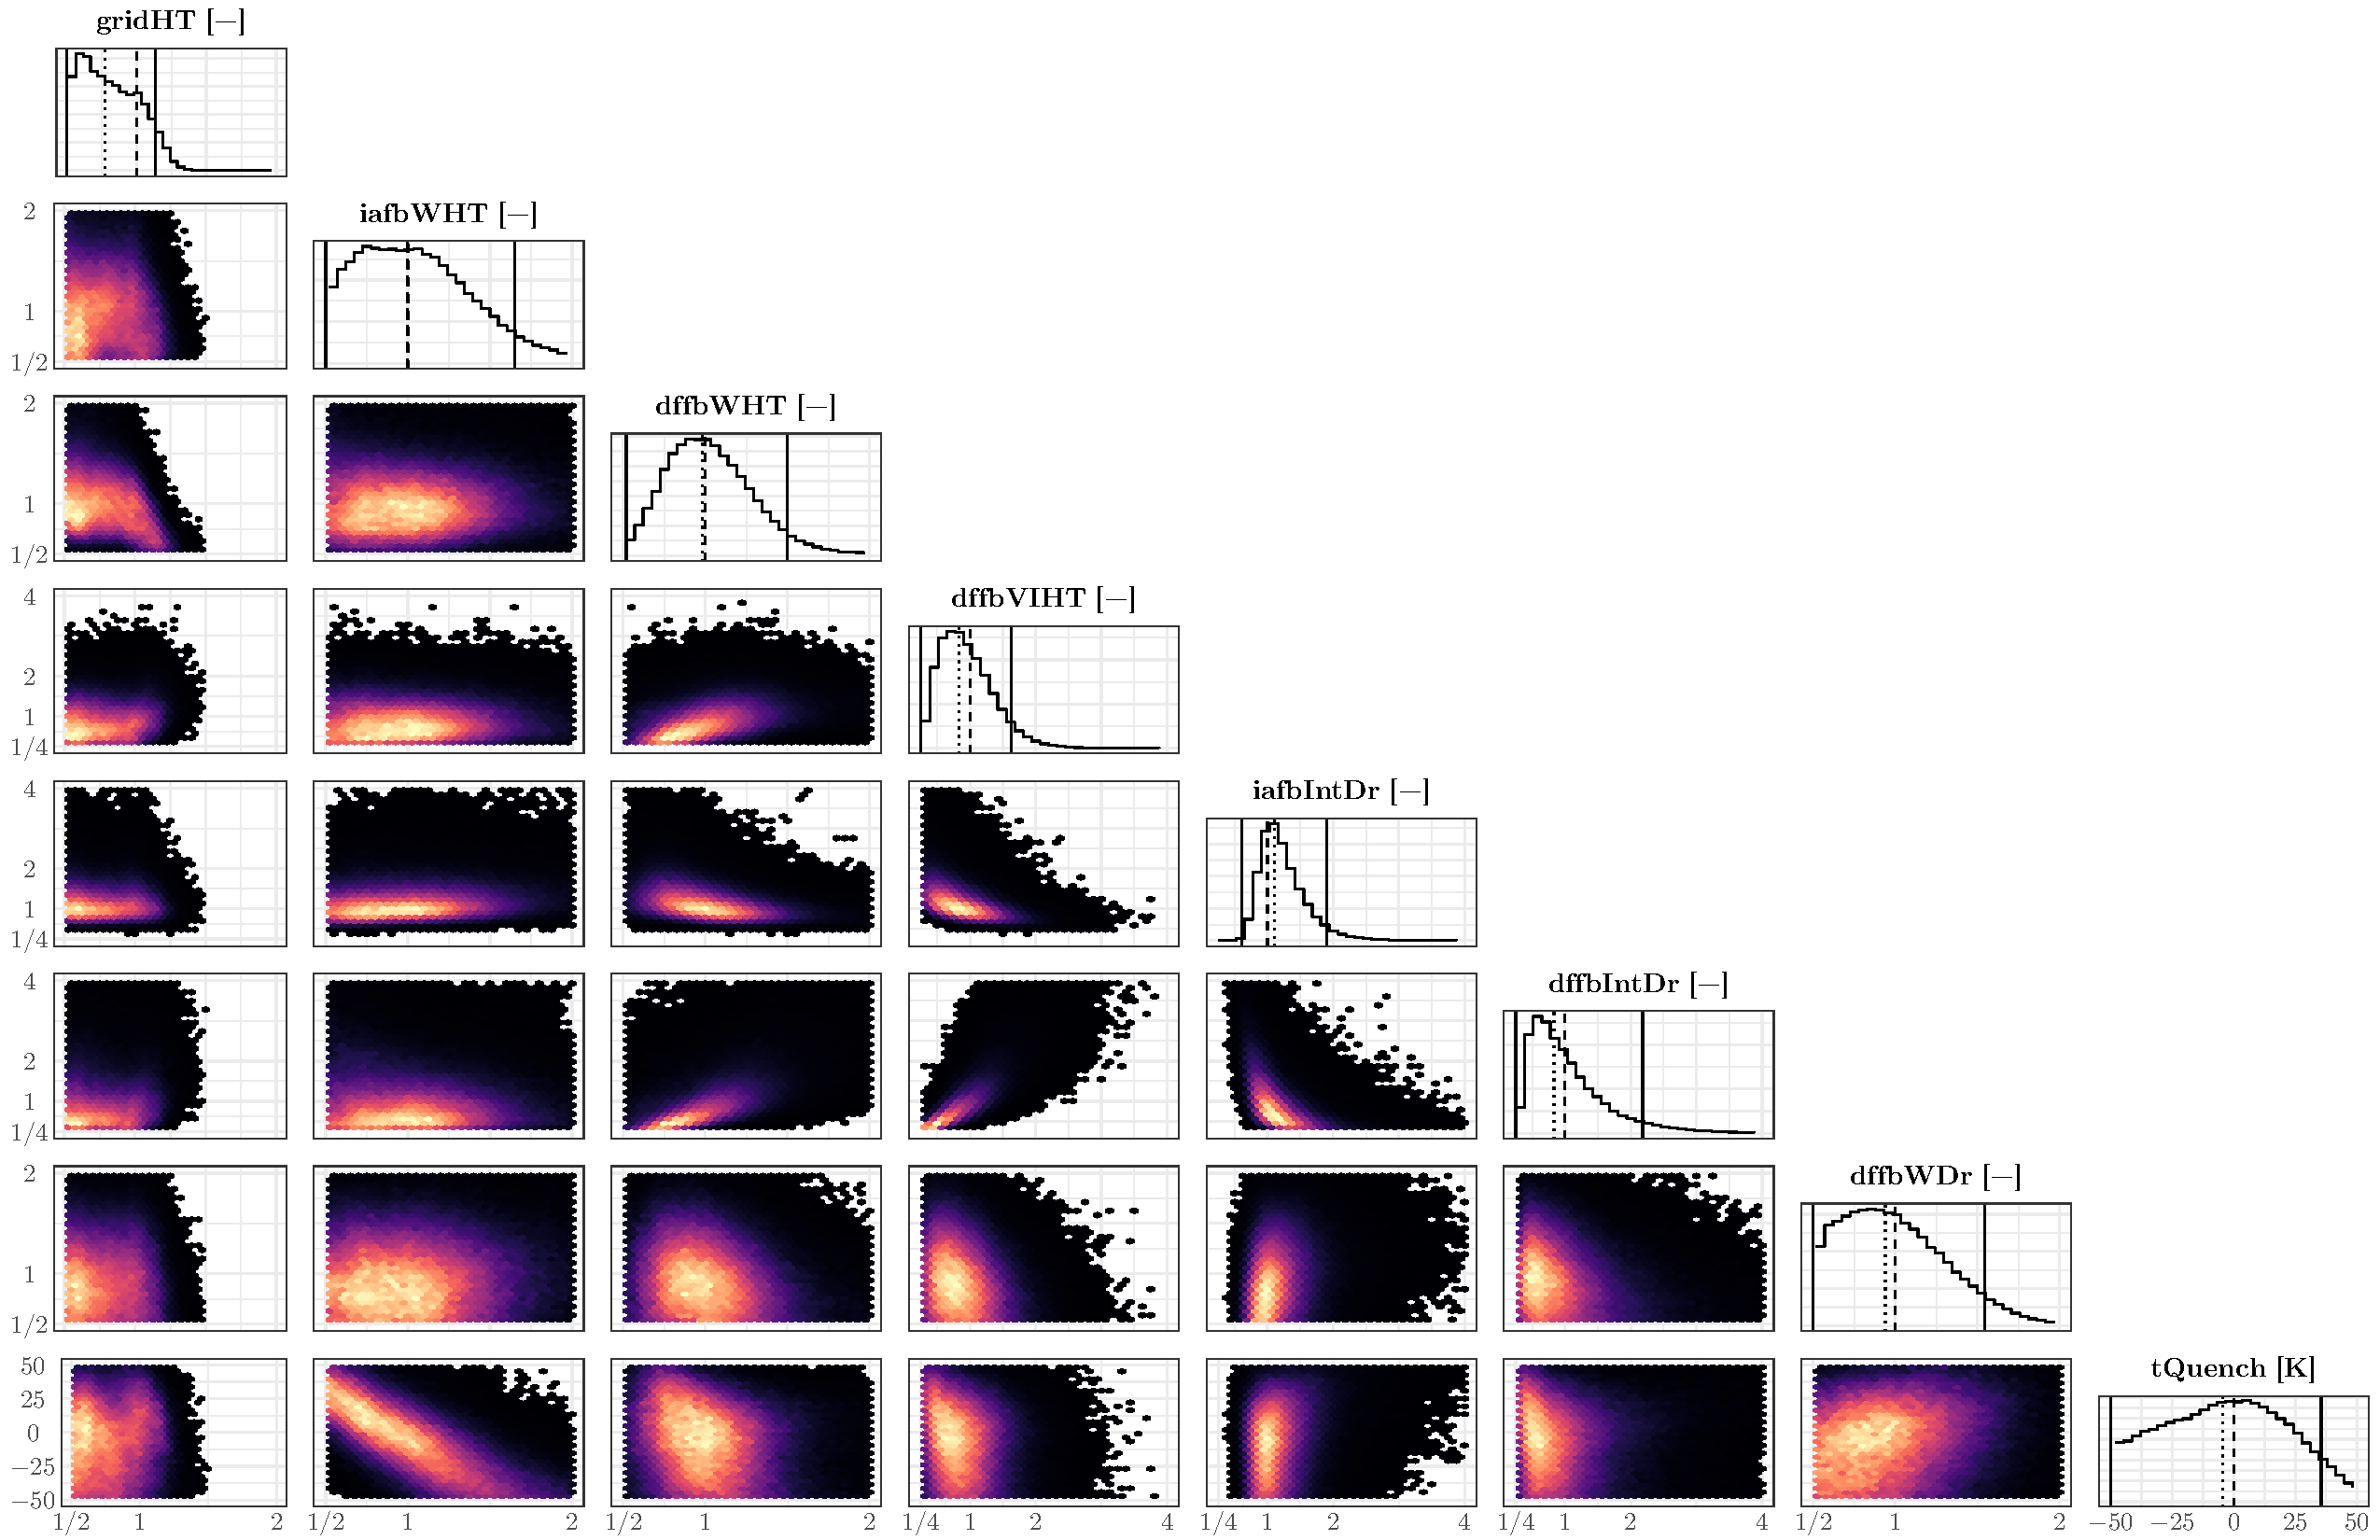
\includegraphics[width=0.90\textwidth]{../figures/chapter5/figures/plotEnsAllDiscCentered}
		\captionof{figure}[Univariate and bivariate marginals of the posterior samples for each of the $8$ model parameters. Calibration with model bias term.]{Univariate and bivariate marginals of the posterior samples for each of the $8$ model parameters. Solid, dashed, and dotted lines indicate the $95\%$ credible intervals, the nominal parameter values, and the posterior median parameter values. Calibration with model bias term.}
	\label{fig:ch5_plot_ens_all_disc_centered}
\end{sidewaysfigure}

% Explaining the figure, bivariate marginal
Although most pairs are largely uncorrelated, the parameter \texttt{dffbIntDr} is strongly correlated with \texttt{dffbWHT}, \texttt{dffbVIHT}, and \texttt{iafbIntDr}.
The parameter \texttt{iafbWHT} is also correlated with \texttt{tQuench}.
Because of the strong correlation between \texttt{dffbVIHT} and \texttt{dffbIntDr}, the calibration scheme \texttt{w/ Bias, no dffbVIHT} was conducted to investigate the effect.
Some correlations (like the one between \texttt{dffbWHT} and \texttt{dffbVIHT}) are approximately elliptical while the others (like the one between \texttt{iafbIntDr} and \texttt{dffbIntDr}) appear more nonlinear.
However, for most of the strongest correlated parameters, regions of high sample density can be identified.
This, in turn, implies that the posterior parameters values that are consistent with the experimental data are largely contained within a small, bounded region of the parameter space, much smaller than the prior parameter space.

% Presenting Table
Table~\ref{tab:ch5_post_param} summarizes the prior and posteriors model parameters uncertainties.
The posteriors presented are from all the calibration schemes considered.
The three numbers inside the brackets correspond to the $2.5$-th percentile, the median (for the prior also the the nominal values), and the lower $97.5$-th percentile, respectively.
That is, the interval constructed by the percentiles corresponds to the symmetric $95\%$ credible interval covering $95\%$ probability.

\begin{sidewaystable}
\caption{Summary of calibration results. The three numbers in brackets are the lower $95\%$ credible interval, the median, and the upper $95\%$ credible interval, respectively.}
\label{tab:ch5_post_param}
\centering
\newcolumntype{Y}{>{\RaggedRight\arraybackslash}X}
\begin{tabularx}{1.025\textwidth}{@{}ccccccccc@{}}
\toprule
\multirow{2}{*}{No.} & \multirow{2}{*}{Parameter} & \multirow{2}{*}{Prior} &    \multicolumn{6}{c}{Posterior Summaries} \\
                                           \cmidrule{4-9}
                   &  ID               &   Summaries                      & \texttt{w/ Bias, All}            &\texttt{w/ Bias, TC}              &\texttt{w/ Bias, DP}              &\texttt{w/ Bias, CO}               &\texttt{w/ Bias, no dffbVIHT}      &\texttt{w/o Bias}\\ \midrule
\footnotesize{$1$} & \texttt{gridHT}   &\footnotesize{$[0.52,1.00,1.93]$} &\footnotesize{$[0.51,0.77,1.18]$} &\footnotesize{$[0.51,0.78,1.28]$} &\footnotesize{$[0.52,0.92,1.82]$} &\footnotesize{$[0.52,0.95,1.91]$}  &\footnotesize{$[0.51,0.80,1.18]$}  &\footnotesize{$[0.50,0.94,1.06]$}\\
\footnotesize{$2$} &\texttt{iafbWHT}   &\footnotesize{$[0.52,1.00,1.93]$} &\footnotesize{$[0.53,1.00,1.77]$} &\footnotesize{$[0.52,0.92,1.83]$} &\footnotesize{$[0.53,1.06,1.92]$} &\footnotesize{$[0.52,0.97,1.92]$}  &\footnotesize{$[0.53,1.02,1.78]$}  &\footnotesize{$[0.50,0.52,1.99]$}\\
\footnotesize{$3$} &\texttt{dffbWHT}   &\footnotesize{$[0.52,1.00,1.93]$} &\footnotesize{$[0.58,0.98,1.61]$} &\footnotesize{$[0.56,0.97,1.71]$} &\footnotesize{$[0.51,0.85,1.88]$} &\footnotesize{$[0.52,0.95,1.93]$}  &\footnotesize{$[0.62,1.06,1.64]$}  &\footnotesize{$[0.50,0.52,0.71]$}\\
\footnotesize{$4$} &\texttt{dffbVIHT}  &\footnotesize{$[0.27,1.00,3.73]$} &\footnotesize{$[0.31,0.83,1.82]$} &\footnotesize{$[0.30,0.90,2.10]$} &\footnotesize{$[0.27,0.92,3.39]$} &\footnotesize{$[0.27,0.75,3.10]$}  &\footnotesize{$[0.27,1.00,3.73]$}  &\footnotesize{$[3.36,3.90,4.00]$}\\
\footnotesize{$5$} &\texttt{iafbIntDr} &\footnotesize{$[0.27,1.00,3.73]$} &\footnotesize{$[0.69,1.10,2.09]$} &\footnotesize{$[0.36,1.27,3.75]$} &\footnotesize{$[0.61,1.11,3.09]$} &\footnotesize{$[0.27,1.03,3.74]$}  &\footnotesize{$[0.70,1.02,1.76]$}  &\footnotesize{$[0.46,0.57,0.71]$}\\
\footnotesize{$6$} &\texttt{dffbIntDr} &\footnotesize{$[0.27,1.00,3.73]$} &\footnotesize{$[0.32,0.83,2.56]$} &\footnotesize{$[0.30,0.97,3.33]$} &\footnotesize{$[0.31,1.17,3.62]$} &\footnotesize{$[0.30,1.22,3.74]$}  &\footnotesize{$[0.57,1.03,1.96]$}  &\footnotesize{$[0.39,0.96,2.23]$}\\
\footnotesize{$7$} &\texttt{dffbWDr}   &\footnotesize{$[0.52,1.00,1.93]$} &\footnotesize{$[0.53,0.94,1.66]$} &\footnotesize{$[0.52,1.01,1.93]$} &\footnotesize{$[0.53,0.97,1.72]$} &\footnotesize{$[0.52,1.01,1.93]$}  &\footnotesize{$[0.52,0.92,1.62]$}  &\footnotesize{$[0.50,0.52,0.62]$}\\
\footnotesize{$8$} &\texttt{tQuench}   &\footnotesize{$[-47.5,0.0,47.5]$} &\footnotesize{$[-47.,-4.6,40.5]$}&\footnotesize{$[-47.8,-8.,42.5]$}&\footnotesize{$[-47.,-3.5,44.8]$}&\footnotesize{$[-47.6,-1.9,47.2]$} &\footnotesize{$[-47.2,-7.7,36.9]$} &\footnotesize{$[-49.7,48.4,50.]$}\\ 
\bottomrule
\end{tabularx}
\end{sidewaystable}

% Explaining the table
From the table, it can be seen that considering additional outputs in the calibration tends to constrain even more the posterior range of the parameters (see also Figs.~\ref{fig:ch5_plot_ens_tc_disc_centered}, \ref{fig:ch5_plot_ens_dp_disc_centered}, and \ref{fig:ch5_plot_ens_co_disc_centered}).
Furthermore, the calibration scheme in which the parameter \texttt{dffbVIHT} was excluded tends to have a tighter posterior uncertainty range for the parameters that were correlated with the parameter \texttt{dffbVIHT} (i.e., \texttt{dffbIntDr} and \texttt{iafbIntDr}),
while the range for the \texttt{dffbVIHT} remains at its initial prior range (see Fig.~\ref{fig:ch5_plot_ens_all_disc_centered_noparam8}).
Finally, the posterior of the calibration scheme without model bias term tends to have a tight range and to be concentrated at either end of the prior range.
Additionally, the median posterior values of the parameters are shifted far away from their initial nominal values.
Most of the initial nominal values actually fall outside the $95\%$ credible intervals (see Fig.~\ref{fig:ch5_plot_ens_all_nodisc}).
